%================================================================
\chapter{O programa E-foto}
%================================================================

Nesse capítulo será apresentado o software E-foto, suas funcionalidades e o que deve ser feito para sua obtenção e instalação. Sendo explicado quais pacotes serão necessários para o funcionamento do programa após a realização do seu download.

\section{O que é o E-foto}
\subsection{O que é e qual o objetivo do E-foto}
De acordo com o site oficial\footnote{\url{http://www.efoto.eng.uerj.br/about-e-foto}}, o E-foto é um software livre para fotogrametria digital que é desenvolvido pelo laboratório de fotogrametria da Universidade do Estado do Rio de Janeiro desde 2004 e tem como objetivo, além da criação de um software inteiramente funcional (uma estação fotogramétrica gratuita), levar aos alunos o conhecimento de forma gratuita sobre fotogrametria digital, sendo de forma didática ou até mesmo na prática por meio de acesso ao código, uso da plataforma e até criação de novos módulos para o software.

\subsection{O que é a fotogrametria}
A fotogrametria remete etimologicamente à ideia da realização de medidas em imagens, e tem como objetivo geral a recriação de parte de um espaço tridimensional a partir de imagens bidimensionais obtidas sem contado entre o sensor e o alvo fotografado. A fotogrametria é classificada de acordo com a evolução dos métodos de obtenção e de análise das imagens, cuja realização deixou de ser analógica e se tornou digital em tempos atuais, aumentando a precisão e a velocidade, e deixando de lado o trabalho mais artesanal e demorado.
Segundo a \textit{American Society for Photogrammetry and Remote Sensing} (ASP, 1980):

\begin{quote}
	``A fotogrametria é a arte, ciência, e tecnologia de obtenção de informações confiáveis sobre os objetos físicos e o meio ambiente por meio de processos de gravação, medição e interpretação de imagens fotográficas e padrões da energia eletromagnética radiante e outros fenômenos.''
\end{quote}

\subsection{Classificações da fotogrametria}
Usando como referência o  livro \textbf{Fotogrametria Digital}, escrito por Luiz Coelho e Jorge Nunes Brito \cite{bib:livrofotogrametria}, publicado pela Editora da Universidade do Estado do Rio de Janeiro, podemos dizer que as classificações da fotogrametria são feitas de maneira histórica. Assim, a \textbf{fotogrametria pioneira} (1840-1900) se deu alguns anos após a invenção da fotografia e com a ideia de usá-la para auxílio na topografia, mas sem grandes resultados, sua utilização começou mesmo a ser difundida em 1851 para documentação de edifícios históricos, sendo criados os seus primeiros métodos de utilização, mas somente com avanços na tecnologia aérea a fotogrametria pôde realmente ser impulsionada e a dificuldade na obtenção de imagens aéreas foi reduzida. 

A \textbf{fotogrametria analógica} (1901-1950) se deu após a primeira revolução da fotogrametria, que ocorre com a invenção do aparelho \textit{estereocomparador} que colocava aparelhos óptico mecânicos no lugar de inúmeros cálculos matemáticos, facilitando a vida dos usuários. Em 1911 foi aumentado o uso de retificadores analógicos devido à criação de um método funcional de retificação de imagens que tornou usual a utilização das fotografias para mapear extensas superfícies. A Alemanha e a Suíça tinham aparelhos que tornavam possíveis a criação de cartas topográficas de alta precisão. Esse avanço na tecnologia da fotogrametria fez com o trabalho se tornasse cada vez mais especializado, assim passou a ter necessidade de um profissional de conhecimento técnico para a realização do mesmo. Paralelamente a esse avanço ocorreram também mais fatos que ajudaram no avanço da fotogrametria em geral, o processo de foto triangulação analógica facilitou o trabalho externo, as câmaras métricas que realizavam impressões de imagens relevantes quanto às coordenadas, o que fez aumentar a precisão das medidas realizadas.

A partir da evolução da tecnologia computacional, grande parte do trabalho manual e mecânico foram substituídos por tarefas feitas diretas no computador dando início a era da \textbf{fotogrametria analítica} (1951-1990). Com o auxílio da computação os cálculos em cima das imagens eram feitos pelos computadores e passou a ter a possibilidade da utilização de conjunto de imagens para serem medidas simultaneamente assim como um estudo mais completo da propagação de erros, passou a ser permitido também a utilização de câmeras não-métricas.

Com o avanço tecnológico ocorreram mudanças bem significativas no quesito de obtenção de imagens, uma vez que com a criação das câmeras digitais ou até mesmo com a utilização de um escâner se pôde obter imagens digitais. Com avanços da computação os computadores passaram a processar essas imagens, com isso surgiu a era da \textbf{fotogrametria digital} (1990-atualmente). Para o processo foram criadas estações com aparelhos específicos para a fotogrametria, as chamadas estações fotogramétricas digitais, nas quais todo o processo é feito por meio de computadores, desde a sua entrada (fotos digitais ou analógicas digitalizadas) até a sua saída (dados digitais compatíveis com programas existentes).

As classificações da fotogrametria ao longo do tempo podem ser observadas na figura \ref{fig:linha_do_tempo}

\begin{figure}[!ht]{17cm}
	\centering
	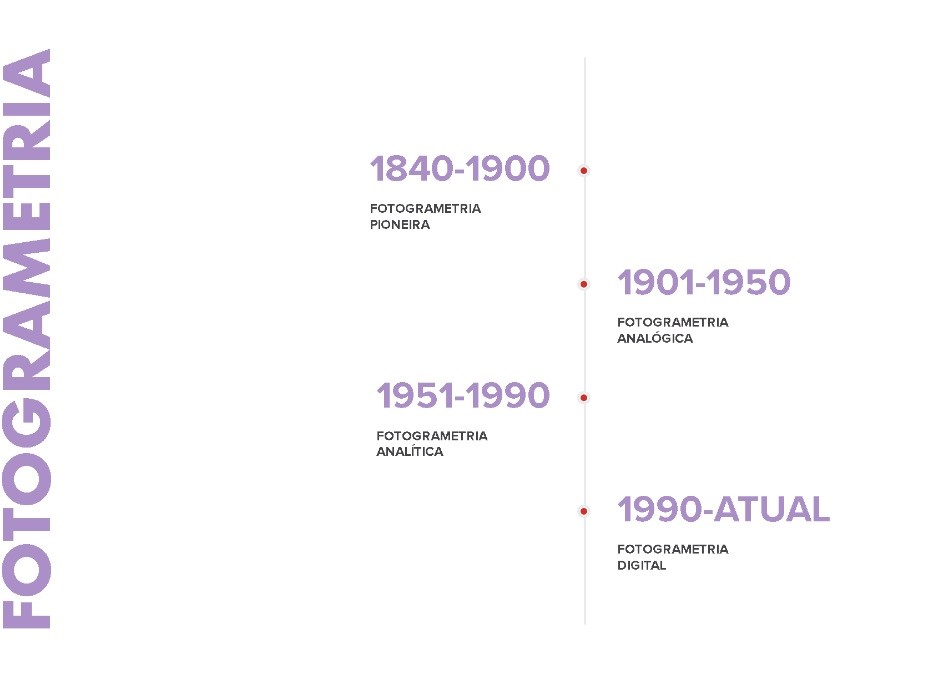
\includegraphics[width=12cm]{Figuras/linha_do_tempo.jpg}
	\caption{Linha do tempo com as classificações da fotogrametria} \label{fig:linha_do_tempo}
\end{figure}

%este paragráfo foi comentado por completo pois é preciso perguntar a um professor sobre a veracidade desses fatos, pois os mesmos são de fontes talvezz ultrapassadas.
%\subsection{Obtenção de imagens fotogramétricas digitais}
%Podemos obter uma imagem fotogramétrica digital de duas maneiras: por meio de escâneres (digitalização de imagens obtidas %analogicamente) e por meio de câmeras fotogramétricas digitais (maneira mais direta). Com a utilização dos escâneres normalmente é %possível obter a melhor configuração para a digitalização desejada, mas mesmo com essa configuração, existe a ocorrência de perda de %alguma informação durante o processo de digitalização, posto que os dispositivos não possuem capacidade de digitalizar toda a %complexidade da imagem. %Por que?

%Essa responsabilidade de configurar os escâneres e seus respectivos programas para que a perda seja menor possível de maneira que a %imagem ainda possa ser utilizada e mantendo a integridade da imagem original é humana, do profissional da área fotogramétrica. No caso %do uso das câmeras fotogramétricas digitais ainda existe muita limitação para seu uso, pois possuem um preço muito elevado. %Isso ainda se mantém? Pesquisar 
%Ainda podem ocorrer problemas na obtenção das imagens devido ao formato das lentes das câmeras, o que também deve ser tratado para %manter a integridade de uma imagem fotogramétrica digital.

\subsection{Importância e os problemas da fotogrametria digital}
A importância da fotogrametria digital é justamente manter o avanço das ferramentas utilizadas para a fotogrametria condizente com os avanços tecnológicos, assim cada vez mais os processos ficam computadorizados e consequentemente mais rápidos e automatizados.

Apesar da tendência a automatizar todo o processo da fotogrametria, proposto pela fotogrametria digital, ainda existe o problema de que as superfícies são muito imperfeitas e possuem inúmeras descontinuidades. Essas descontinuidades dificultam bastante a obtenção de valores razoáveis automaticamente mapeados. Assim, a participação humana se faz necessária, mesmo que só para supervisionar a qualidade do que está sendo mapeado, tornando o trabalho semiautomático ou o mais automático possível, tentando não comprometer a qualidade do processo.


\section{Utilização do E-foto}

A importância do E-foto e suas vantagens vêm desde a sua criação, pois a mesma promove um encontro entre campos diferentes da engenharia e suas especialidades, sendo eles a \textbf{engenharia de computação} e a \textbf{engenharia cartográfica}, gerando assim um conhecimento, mesmo que básico, do que pode ser feito em uma área que não é necessariamente a especialidade do aluno ou usuário. Outra vantagem vem da possibilidade de colocar em prática determinados assuntos que são vistos de forma teórica em sala de aula ou em livros em ambas as vertentes da engenharia, o que por muitas vezes não é feito durante a graduação e quando é feito, raramente é com algo de tamanha importância quanto o E-foto. O E-foto é uma estação fotogramétrica digital que tem acesso público e gratuito, de modo que a qualidade da sua criação tem grande impacto em sua utilização, e essa qualidade é exigida pelos professores criadores, já que os mesmos prezam bastante por isso, assim como a instituição de ensino como um todo.

\section{Instalação do E-foto}

\subsection{Em Sistemas Linux}

\subsubsection{Passo 1 - Baixar o .deb do website}

Para a instalação do e-foto em sistemas Linux, o usuário deverá fazer o \textit{download} e instalação a partir do arquivo \textit{.deb}\footnote{Disponível em  \url{http://www.efoto.eng.uerj.br/download/latest-version}}, escolhendo a opção designada para Ubuntu/Linux na aba \textbf{latest version}.

\subsubsection{Passo 2 - Instalar o pacote baixado da versão 2016.06.425}

Para realizar a instalação da versão 2016.06.425 do E-foto que é a disponibilizada atualmente pelo site,  basta após realizar o download utilizar o comando:

\begin{lstlisting}[language=bash]
	$ sudo dpkg -i nome_do_pacote
\end{lstlisting}

Após isso, é necessário buscar o caminho do diretório onde o E-foto foi instalado através do terminal e utilizar o comando:

\begin{lstlisting}[language=bash]
	$ ./efoto
\end{lstlisting}

no diretório onde fica o executável, geralmente \textit{usr/bin} é o caminho correto. Seguindo esses passos o E-foto executará corretamente.

\subsection{Em Sistemas Windows}

\subsubsection{Passo 1 - Baixar o instalador do website}
Para instalações em sistemas Windows o usuário irá instalar o E-foto por meio do download e instalação a partir do arquivo .msi e para isso será pode acessar o site \url{http://www.efoto.eng.uerj.br/download/latest-version} e realizar o download da opção designada para Windows na aba \textbf{latest version} como é mostrado na Figura \ref{fig:downmsi}.

\begin{figure}[!ht]{17cm}
	\centering
	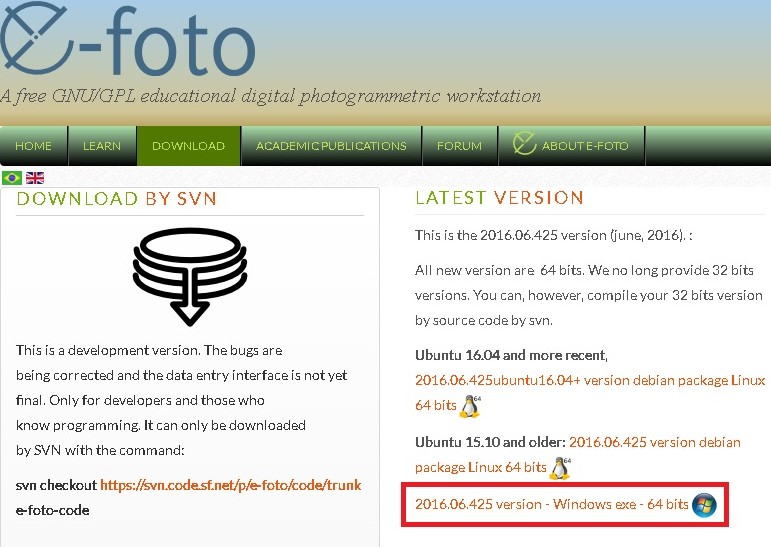
\includegraphics[width=10cm]{Figuras/downmsi.jpg} 
	\caption{Realizando download do instalador do E-foto} \label{fig:downmsi}
\end{figure}

\subsubsection{Passo 2 - Realizar a instalação}
Normalmente o arquivo baixado vai para a pasta \textit{Downloads} do computador do usuário e para realizar a instalação basta dar um clique duplo nesse arquivo, clicar na opção \textit{Next}, ler e aceitar os termos do contrato, e clicar novamente em \textit{Next}.  No próximo passo o usuário deve escolher o caminho onde o E-foto será instalado. Depois o usuário deve clicar em \textit{Install} e a instalação será realizada automaticamente, conforme a Figura \ref{fig:installmsi}.
 
\begin{figure}[!ht]{17cm}
   \centering
   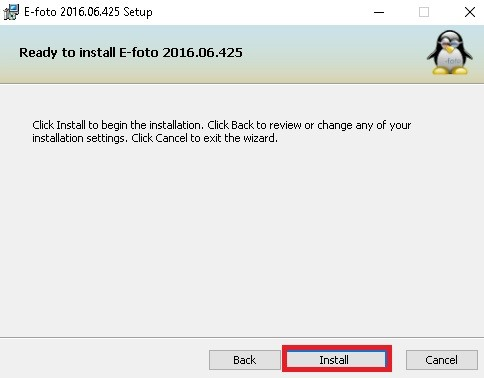
\includegraphics[width=10cm]{Figuras/installmsi.jpg}
   \caption{Instalando E-foto por meio do instalador} \label{fig:installmsi}
\end{figure}
  
\subsubsection{Passo 3 - Executar o programa E-foto}
Após a instalação terminar, basta manter a opção \textit{launch} E-foto e clicar na opção \textit{Finish}, como mostra a Figura \ref{fig:launch1} que o E-foto será executado, ou fechar o instalador e buscar o E-foto nos seus aplicativos instalados, conforme a Figura \ref{fig:launch2}. Neste formato o instalador do E-foto instalará tudo o que é necessário para o seu funcionamento, sem a necessidade de configurações adicionais.

\begin{figure}[!ht]{17cm}
	\centering
	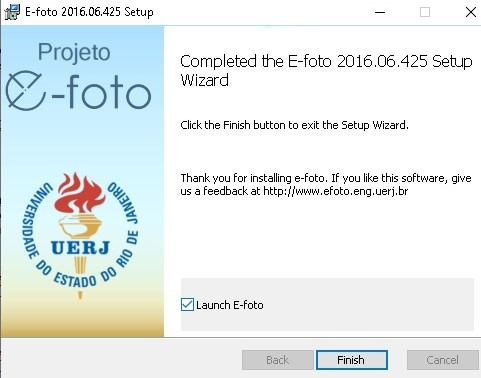
\includegraphics[width=10cm]{Figuras/launch1.jpg}
	\caption{Executando o E-foto pelo instalador} \label{fig:launch1}
\end{figure}

\begin{figure}[!ht]{17cm}
	\centering
	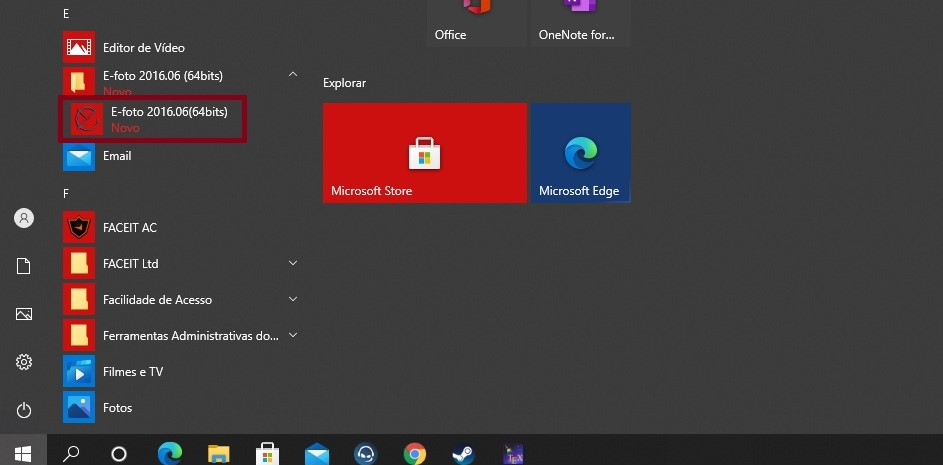
\includegraphics[width=12cm]{Figuras/launch2.jpg}
	\caption{Buscando E-foto nos aplicativos} \label{fig:launch2}
\end{figure}

\subsection{Compilação do E-foto a partir dos fontes}
\subsection{Em Sistemas Linux}

\subsubsection{Passo 1 - Baixar código fonte}
Primeiramente, para realizar a instalação do software E-foto, o usuário pode fazer o download do seu código fonte e para isso é necessário a instalação do \textbf{subversion}, se já não estiver instalado. Para tal, o usuário deve abrir o terminal do seu sistema Linux, que pode ser feito digitando terminal na barra de busca ao apertar a tecla do \textit{Windows} no seu teclado ou pelo atalho do teclado \texttt{ctrl + alt + T}. Com o terminal aberto, o usuário começará a instalação do SVN com os comandos: 
\begin{lstlisting}[language=bash]
	$ sudo apt update
	$ sudo apt install subversion
\end{lstlisting}

Com o SVN instalado e configurado, basta o usuário digitar no terminal o comando:
\begin{lstlisting}[language=bash]
	$ svn checkout https://svn.code.sf.net/p/e-foto/code
\end{lstlisting}

Com a utilização desse comando o download de todo o código fonte do software E-foto será feito automaticamente. 

Também é possível obter o código fonte por download direto através do comando no terminal:

\begin{lstlisting}[language=bash]
	$ wget https://sourceforge.net/p/e-foto/code/HEAD/tree/
\end{lstlisting}
 
\subsubsection{Passo 2 - Instalar pacotes necessários à compilação}  

Após a realização do download do código fonte do E-foto, o usuário deve ficar atento aos pacotes necessários em seu ambiente para que o E-foto possa ser instalado e ter seu funcionamento sem erros. Para a instalação dos pacotes o usuário deve buscar abrir novamente o terminal. Os pacotes necessários para instalação do e-foto são:

\begin{itemize}
   	\item libgdal.dev
   	\item build-essential
   	\item libfontconfig1
   	\item mesa-common-dev
   	\item libx11-xcb-dev
   	\item libglu1-mesa-dev
\end{itemize}
Esses pacotes devem ser instalados com o seguinte comando: 
\begin{lstlisting}[language=bash]
	$ sudo apt install libgdal-dev build-essential libfontconfig1 mesa-common-dev libx11-xcb-dev libglu1-mesa-dev
\end{lstlisting}				
	
O pacote \textit{libgdal.dev} contém as funcionalidades da GDAL, onde GDAL é uma biblioteca de tradução para formatos geoespaciais. Ou seja, como pode ser visto no site\footnote{\url{https://gdal.org/programs/gdal_translate.html}} pode ser usado para converter dados raster (compostos por linhas e colucas de pixels) entre formatos diferentes, potencialmente realizando algumas operações como subconjuntos, reamostragem e redimensionamento de pixels no processo.
O pacote \textit{libfontconfig1} contém uma biblioteca projetada para achar fontes no sistema e selecioná-las de acordo com os requisitos especificados pelas aplicações, e o usuário deve instalar o driver \textbf{XCB} e o \textbf{OpenGl} por meio dos pacotes \textit{mesa-common-dev}, \textit{libx11-xcb-dev} e \textit{libglu1-mesa-dev}. De acordo com o site\footnote{\url{https://www.debian.org/distrib/packages\#search\_packages}}, esses pacotes servem respectivamente para incluir as especificações para as extensões OpenGL específicas do Mesa, o conjunto completo de notas de versão e os arquivos de cabeçalho de desenvolvimento comuns a todos os pacotes do Mesa. Fornecer uma interface de cliente para o X Window System, também conhecido como 'Xlib', fornecendo uma API completa para as funções básicas do sistema de janelas. E fornecer o ambiente de desenvolvimento necessário para compilar programas com a biblioteca de widgets Mesa, libGLw, que serve para que aplicações baseadas em Motif embarquem contexto de desenho OpenGL, incluindo os cabeçalhos e bibliotecas estáticas para compilar programas que usam esta biblioteca.
  
\subsection{Passo 3 - Instalar os pacotes de instalação do Qt 5}   
A instalação do Qt 5 via terminal deve ser feita por meio dos seguintes pacotes:
\begin{itemize}
	\item qt5-default
	\item qt5-qmake
\end{itemize}   
Esses pacotes devem ser instalados por meio dos seguintes comandos do terminal:
\begin{lstlisting}[language=bash]
	$ sudo apt install qt5-default
	$ sudo apt install -y qt5-qmake
\end{lstlisting}	
    
Após esses procedimentos o usuário ja terá um ambiente de compilação pronto para a instalação do E-foto, assim como o plataforma em que o mesmo foi desenvolvido.
    
\subsection{Passo 4 - Compilar e executar o software E-foto}
Para compilar e executar o código do E-foto via terminal, após a realização de todos os passos necessários, o usuário deve utilizar os seguintes comandos no terminal:
\begin{lstlisting}[language=bash]
   	$ cd diretório/
   	$ qmake e-foto.pro
   	$ make
   	$ ./build/bin/e-foto
\end{lstlisting}
   
O comando \textit{cd diretório/} servirá para o usuário percorrer o caminho até o diretório onde está o arquivo \textbf{e-foto.pro} (atualmente \textit{code/branches/e-foto-trunk-candidate}), depois o \textit{qmake} e o \textit{make} irão realizar a compilação e gerar o executável do E-foto. Por fim o último comando irá executar o programa.

\subsection{Em Sistemas Windows}

\subsubsection{Passo 1 - Baixar código fonte}
Para começar a instalação do E-foto em sistemas \textit{Windows}, o usuário deve realizar o download do código fonte do E-foto e para isso o melhor caminho é utilizar o \textit{subversion}, que no \textit{Windows} pode ser feito através de um programa chamado \textbf{TortoiseSVN}, cuja versão usada para essa explicação foi a 1.14.0, e que pode ser baixado gratuitamente por esse link \url{https://tortoisesvn.net/downloads.html} na opção mostrada na Figura \ref{fig:tortoise}. Após a instalação do \textbf{TortoiseSVN}, o usuário deve buscar no programa a opção de SVN Checkout, que pode ser encontrada ao clicar o botão direito do mouse na área de trabalho conforme, é mostrado na figura \ref{fig:checkout} e no espaço para colar uma URL (primeira opção disponível) colocar \url{https://svn.code.sf.net/p/e-foto/code}, como é visto na Figura \ref{fig:url}. Isso deve gerar o download de todo o código fonte do E-foto.

Também existe a opção de baixar o código fonte diretamente do site, basta acessar o endereço \url {https://sourceforge.net/p/e-foto/code/HEAD/tree/} e clicar na opção \textbf{Download Snapshot}.
 
\begin{figure}[!ht]{17cm}
 	\centering
 	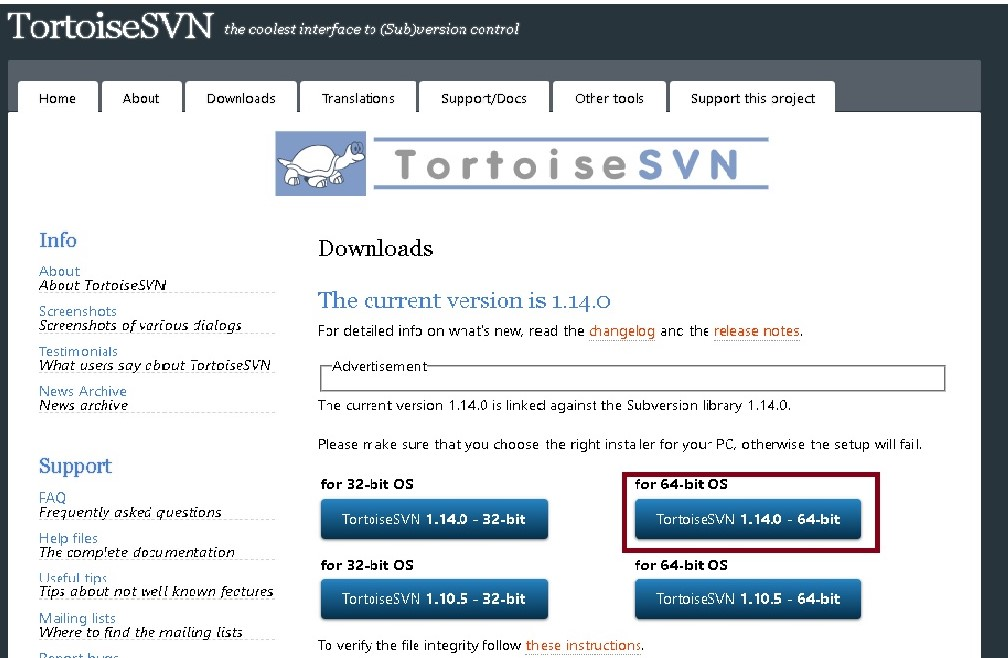
\includegraphics[width=12cm]{Figuras/tortoise.jpg}
 	\caption{Download do TortoiseSVN} \label{fig:tortoise}
\end{figure}

\begin{figure}[!ht]{17cm}
	\centering
	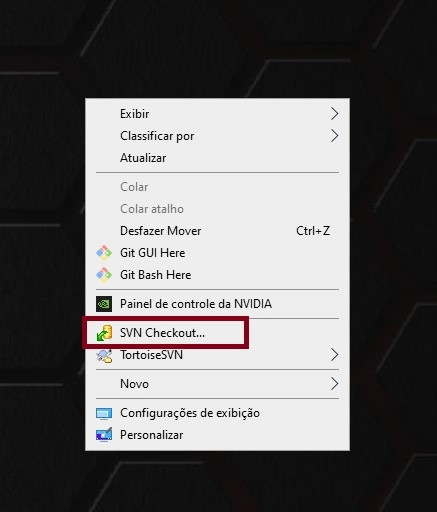
\includegraphics[width=10cm]{Figuras/checkout.jpg}
	\caption{Buscando a opção de checkout} \label{fig:checkout}
\end{figure}

\begin{figure}[!ht]{17cm}
	\centering
	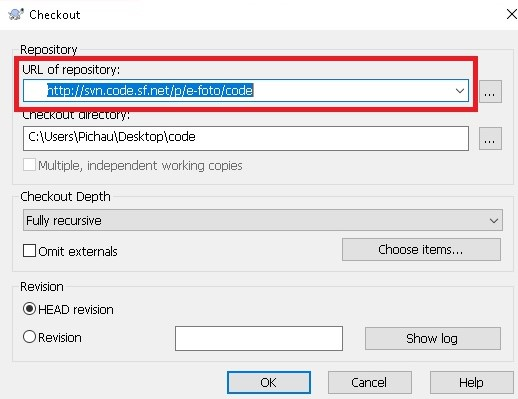
\includegraphics[width=12cm]{Figuras/url.jpg}
	\caption{Realizando o download com a URL} \label{fig:url}
\end{figure}
 
\subsubsection{Passo 2 - Download dos pacotes binários da Gdal no Windows} 
O próximo passo é o download dos pacotes binários da Gdal no \textit{Windows}. Isso pode ser realizado diretamente pelo link  \url{https://repo.msys2.org/distrib/x86\_64/msys2-x86\_64-20200720.exe}, que realizará o download do MSYS. Após a conclusão do download e da instalação do MSYS (que deve ser feita no drive C, que normalmente é o \textit{default}) o usuário deve executar \textbf{mSYS}, o que vai abrir o terminal do próprio MSYS que contém uma versão portada do gerenciador de pacotes \textit{Pacman} conforme pode ser visto na Figura \ref{fig:terminalgdal}. Nessa última versão do \textit{Pacman} deve ser digitado no terminal o comando:

\begin{lstlisting}[language=bash]
$ pacman -Syuu
\end{lstlisting}
 
\begin{figure}[!ht]{17cm}
 	\centering
 	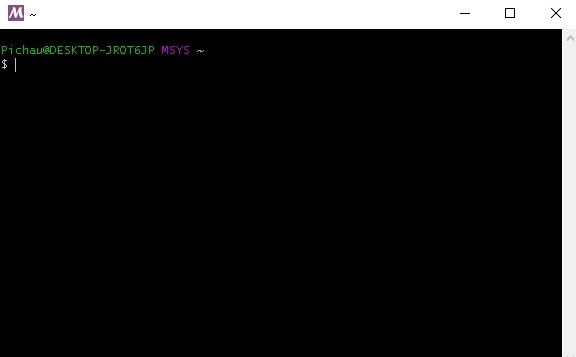
\includegraphics[width=12cm]{Figuras/terminalgdal.jpg}
 	\caption{Terminal MSYS} \label{fig:terminalgdal}
\end{figure}
 

Esse comando irá gerar uma série de instruções a serem seguidas até que o usuário possa repetir o comando e receber a mensagem de que nada necessita ser atualizado. Com o ambiente atualizado, o usuário deve digitar o seguinte comando:
\begin{lstlisting}[language=bash]
 	$ pacman -S mingw64/mingw-w64-x86\_64-gdal
 	$ gdalinfo --version
\end{lstlisting}

Esses comandos realizarão finalmente o download e instalação dos pacotes binários da GDAL e dirão qual versão que foi instalado, respectivamente. 
 
\subsubsection{Passo 3 - Baixar e configurar o Qt 5 e o Qt Creator}
Nessa etapa o usuário pode realizar o download do \textbf{Qt 5} e do \textbf{Qtcreator} no website do Qt\footnote{\url{https://www.qt.io/download}}, como mostrado na Figura \ref{fig:downqt}, deixando claro que na parte da instalação deve ser escolhido para instalar apenas as opções do \textit{mingw} 64-bits, e o Qt 5 referente a esse sistema (Figura \ref{fig:qtinstallconfig}). Com os arquivos do código fonte do E-foto disponíveis, o usuário deve procurar no caminho \textit{e-foto-code/branches/e-foto-trunk-candidate} por um arquivo chamado \textbf{e-foto.pro}, como mostrado na Figura \ref{fig:openpro}. Quando abrir o projeto no \textit{Qtcreator} será necessário configurar o que deverá ser usado, começando pela escolha do kit que será usado, que deve ser o mesmo escolhido na instalação do Qt 5, ou seja, o \textit{mingw} 64-bits e a versão do Qt referente a esse sistema, como mostra a Figura \ref{fig:qtkit}. Após o projeto estar aberto, o usuário deve ir na guia \textit{project} e desmarcar a opção \textit{shadow build}, e depois procurar e clicar na aba \textbf{build} a opção \textit{build E-foto}. Quando acabar a compilação é só clicar na opção \textbf{Run}, que também pode ser encontrado na aba \textit{build}, e o E-foto vai abrir pronto para o uso como está assinalado na Figura \ref{fig:projectbuild}.
\begin{figure}[!ht]{17cm}
  	\centering
 	
\includegraphics[width=12cm]{Figuras/downqt.jpg}
 	\caption{Download do Qt 5 pelo website} \label{fig:downqt}
\end{figure}

\begin{figure}[!ht]{17cm}
 	\centering
	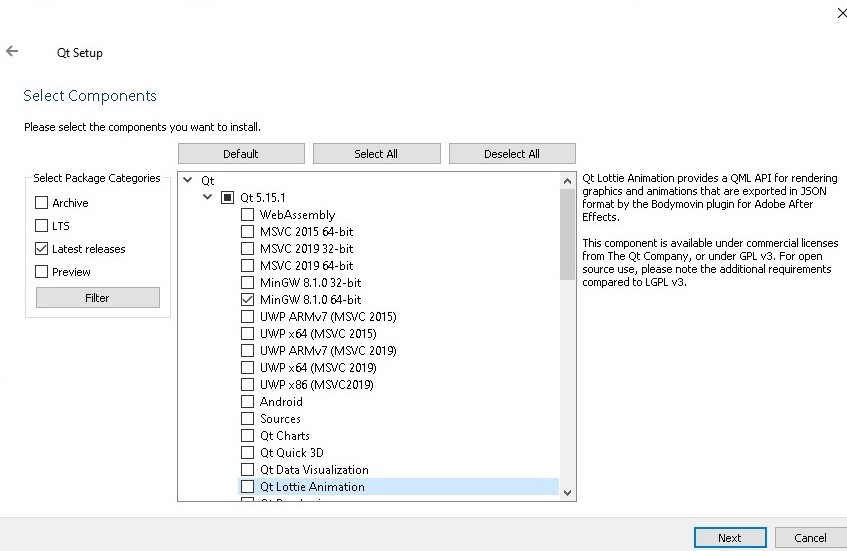
\includegraphics[width=12cm]{Figuras/qtinstallconfig.jpg}
	\caption{Configuração da instalação do Qt 5} \label{fig:qtinstallconfig}
\end{figure}

\begin{figure}[!ht]{17cm}
 	\centering
	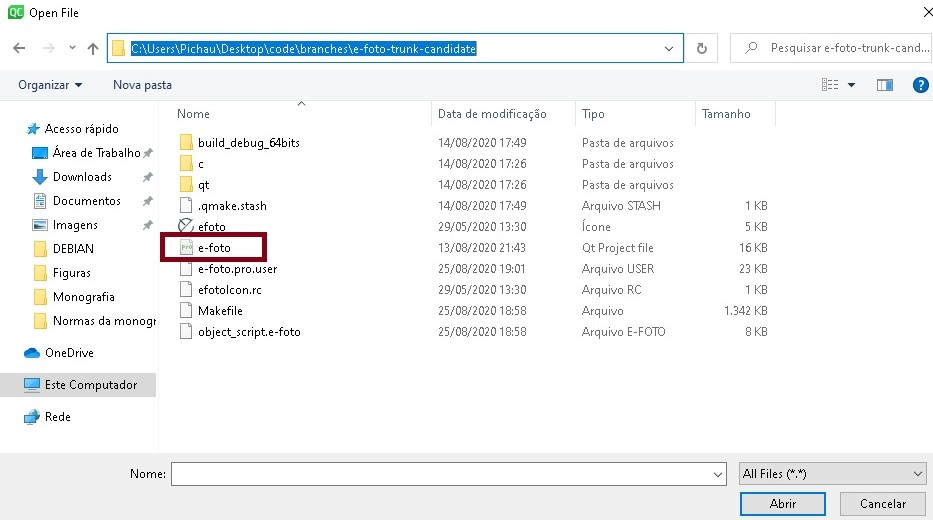
\includegraphics[width=15cm]{Figuras/openpro.jpg}
	\caption{Caminho do arquivo do projeto E-foto} \label{fig:openpro}
\end{figure}

\begin{figure}[!ht]{17cm}
 	\centering
	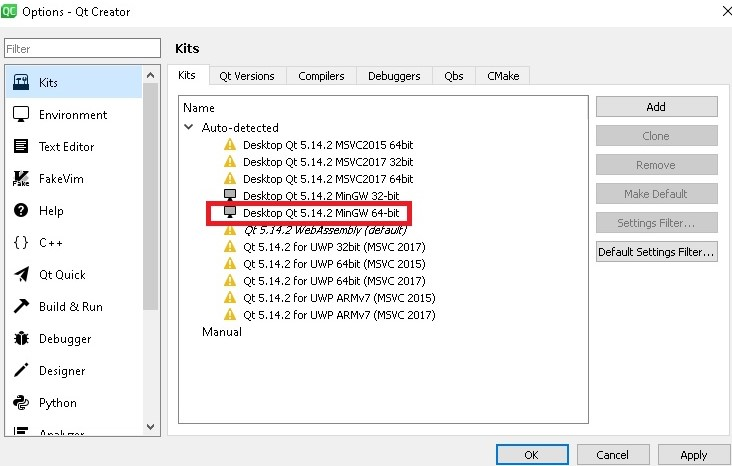
\includegraphics[width=15cm]{Figuras/qtkit.jpg}
	\caption{Configuração do kit} \label{fig:qtkit}
\end{figure}

\begin{figure}[!ht]{17cm}
 	\centering
	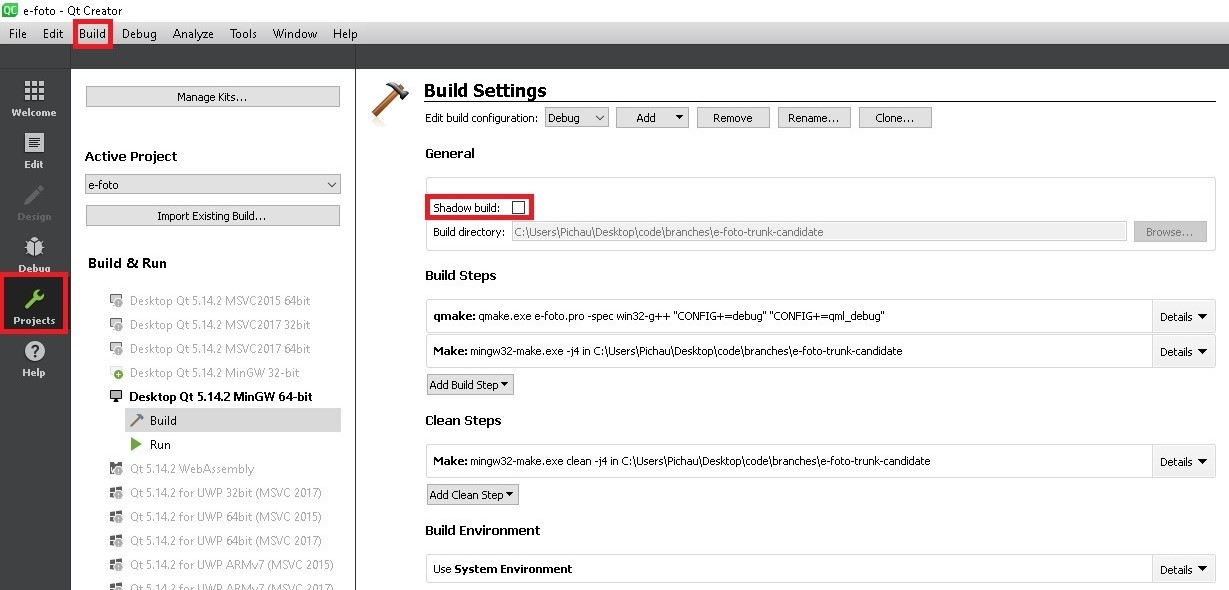
\includegraphics[width=15cm]{Figuras/projectbuild.jpg}
	\caption{Locais buscados para a compilação} \label{fig:projectbuild}
\end{figure}
 